\documentclass{ximera}

\input{../../../preamble.tex}


\definecolor{fvdnavy}{HTML}{071D43}
\definecolor{fvdcyan}{HTML}{20BFC6}
\definecolor{fvdcyanlight}{HTML}{EFFCFB}
\definecolor{fvdmagenta}{HTML}{F10D69}
\definecolor{fvdmagentalight}{HTML}{FFF1F7}
\definecolor{fvdtext}{HTML}{163044}





%=================================================
% Pedagogische omgevingen
% PDF: tcolorbox
% HTML: learning-box
%=================================================

\newenvironment{voorkennis}
{%
    \ifdefined\HCode
        \HCode{%
<section class="learning-box learning-box--prior">
<div class="learning-box__header">
<span class="learning-box__icon" aria-hidden="true"></span>
<span class="learning-box__title">Voorkennis</span>
</div>
<div class="learning-box__content">
        }%
        \begin{itemize}
    \else
       \begin{tcolorbox}[
    enhanced,
    breakable,
    colback=fvdcyanlight,
    colframe=fvdcyan,
    coltext=fvdtext,
    boxrule=0.5pt,
    leftrule=4pt,
    arc=4mm,
    outer arc=4mm,
    left=7mm,
    right=6mm,
    top=5mm,
    bottom=5mm,
    before skip=6mm,
    after skip=6mm,
    title=Voorkennis,
    coltitle=fvdcyan,
    fonttitle=\bfseries\Large,
    attach title to upper={\par\smallskip},
    boxed title style={
        empty,
        left=0mm,
        right=0mm,
        top=0mm,
        bottom=0mm
    },
    overlay={
        \draw[
            fvdcyan,
            line width=0.5pt
        ]
        ([xshift=42mm,yshift=-13mm]frame.north west)
        --
        ([xshift=-7mm,yshift=-13mm]frame.north east);
    }
]
        \begin{itemize}
    \fi
}
{%
    \end{itemize}
    \ifdefined\HCode
        \HCode{%
</div>
</section>
        }%
    \else
        \end{tcolorbox}
    \fi
}


\newenvironment{leerdoelen}
{%
    \ifdefined\HCode
        \HCode{%
<section class="learning-box learning-box--goals">
<div class="learning-box__header">
<span class="learning-box__icon" aria-hidden="true"></span>
<span class="learning-box__title">Leerdoelen</span>
</div>
<div class="learning-box__content">
        }%
        \begin{itemize}
    \else
\begin{tcolorbox}[
    enhanced,
    breakable,
    colback=fvdmagentalight,
    colframe=fvdmagenta,
    coltext=fvdtext,
    boxrule=0.5pt,
    leftrule=4pt,
    arc=4mm,
    outer arc=4mm,
    left=7mm,
    right=6mm,
    top=5mm,
    bottom=5mm,
    before skip=6mm,
    after skip=6mm,
    title=Leerdoelen,
    coltitle=fvdmagenta,
    fonttitle=\bfseries\Large,
    attach title to upper={\par\smallskip},
    boxed title style={
        empty,
        left=0mm,
        right=0mm,
        top=0mm,
        bottom=0mm
    },
    overlay={
        \draw[
            fvdmagenta,
            line width=0.5pt
        ]
        ([xshift=42mm,yshift=-13mm]frame.north west)
        --
        ([xshift=-7mm,yshift=-13mm]frame.north east);
    }
]
        \begin{itemize}
    \fi
}
{%
    \end{itemize}
    \ifdefined\HCode
        \HCode{%
</div>
</section>
        }%
    \else
        \end{tcolorbox}
    \fi
}



\title{Symmetrie — even en oneven functies}
\author{Ingmar Herreman}

\begin{document}

\fvdchapterdata{5}{Het gedrag van functies beschrijven}{4}

\begin{abstract}
Symmetrie maakt het mogelijk om uit een deel van een grafiek informatie over
de rest af te leiden. We onderzoeken symmetrie ten opzichte van de \(y\)-as
en de oorsprong en verbinden die grafische kenmerken met de voorwaarden
\(f(-x)=f(x)\) en \(f(-x)=-f(x)\).
\end{abstract}

\maketitle

\begin{voorkennis}
Je kunt:
\begin{itemize}
  \item punten en grafieken in een assenstelsel interpreteren;
  \item functiewaarden \(f(a)\) en \(f(-a)\) bepalen;
  \item een functievoorschrift invullen en vereenvoudigen;
  \item domein en grafische kenmerken van een functie onderzoeken.
\end{itemize}
\end{voorkennis}

\begin{leerdoelen}
Na dit hoofdstuk kun je:
\begin{itemize}
  \item symmetrie ten opzichte van de \(y\)-as en de oorsprong grafisch herkennen;
  \item het verband leggen tussen \(f(-x)=f(x)\) en even functies;
  \item het verband leggen tussen \(f(-x)=-f(x)\) en oneven functies;
  \item met een voorschrift onderzoeken of een functie even, oneven of geen van beide is;
  \item vanuit symmetrie ontbrekende grafische informatie reconstrueren;
  \item gevolgen van symmetrie voor functiewaarden en bijzondere punten afleiden;
  \item rekening houden met het domein bij uitspraken over evenheid en onevenheid;
  \item symmetrie doelgericht gebruiken om een functie efficiënter te analyseren.
\end{itemize}
\end{leerdoelen}

\FVDsection{Symmetrie in een grafiek}

Sommige grafieken bevatten herhaling door spiegeling of puntspiegeling.
Daardoor hoeft niet elk deel van de grafiek afzonderlijk onderzocht te worden.

Vergelijk de functies
\[
f(x)=x^2
\qquad\text{en}\qquad
g(x)=x^3.
\]

\begin{center}
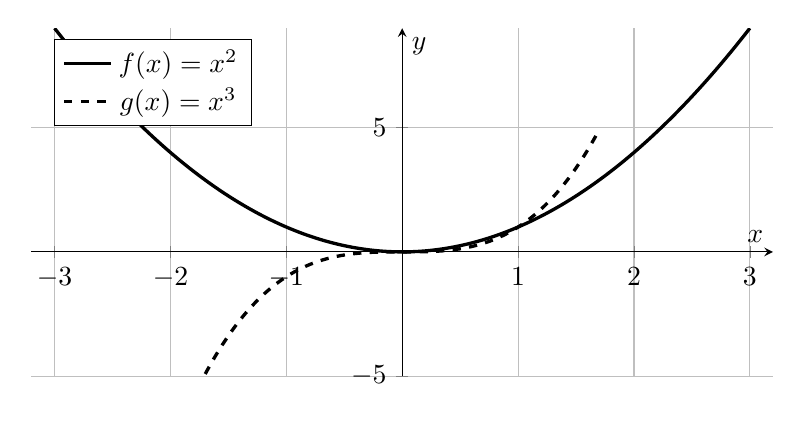
\begin{tikzpicture}
\begin{axis}[
 width=11cm,height=6cm,
 axis lines=middle,
 xmin=-3.2,xmax=3.2,ymin=-5,ymax=9,
 xlabel={$x$},ylabel={$y$},
 grid=both,samples=200,
 legend style={at={(0.03,0.97)},anchor=north west}
]
\addplot[very thick,domain=-3:3] {x^2};
\addlegendentry{\(f(x)=x^2\)}
\addplot[very thick,dashed,domain=-1.7:1.7] {x^3};
\addlegendentry{\(g(x)=x^3\)}
\end{axis}
\end{tikzpicture}
\end{center}

De grafiek van \(x^2\) is gespiegeld ten opzichte van de \(y\)-as.
De grafiek van \(x^3\) blijft onveranderd bij een puntspiegeling in de oorsprong.

Deze twee vormen van symmetrie leiden tot \textbf{even} en \textbf{oneven} functies.

\FVDsection{Even functies}

\begin{definitie}
Een functie \(f\) is \textbf{even} als voor elke \(x\) uit haar domein ook
\(-x\) tot het domein behoort en
\[
\boxed{f(-x)=f(x).}
\]
\end{definitie}

Grafisch betekent dit dat de grafiek symmetrisch is ten opzichte van de \(y\)-as.

Als
\[
(a,f(a))
\]
op de grafiek ligt, dan ligt ook
\[
(-a,f(a))
\]
op de grafiek.

\begin{center}
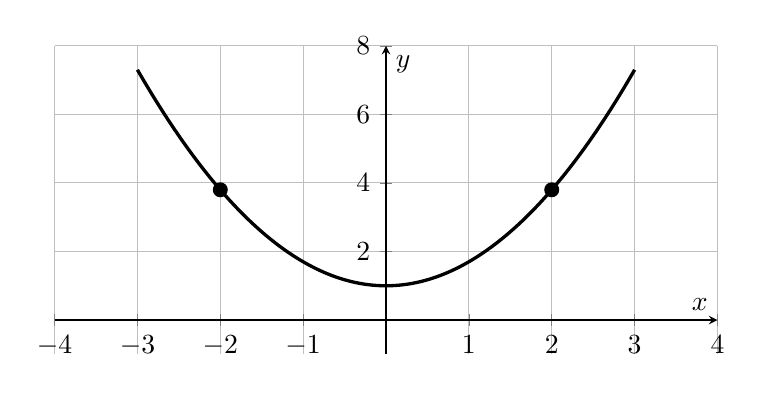
\begin{tikzpicture}
\begin{axis}[
 width=10cm,height=5.5cm,
 axis lines=middle,
 xmin=-4,xmax=4,ymin=-1,ymax=8,
 xlabel={$x$},ylabel={$y$},
 grid=both,samples=200
]
\addplot[very thick,domain=-3:3] {0.7*x^2+1};
\addplot[only marks,mark=*,mark size=2.5pt]
coordinates {(-2,3.8) (2,3.8)};
\end{axis}
\end{tikzpicture}
\end{center}

\begin{voorbeeld}
Voor
\[
f(x)=x^4+2x^2-3
\]
geldt
\[
f(-x)=(-x)^4+2(-x)^2-3=x^4+2x^2-3=f(x).
\]
Dus \(f\) is even.
\end{voorbeeld}

\FVDsection{Oneven functies}

\begin{definitie}
Een functie \(f\) is \textbf{oneven} als voor elke \(x\) uit haar domein ook
\(-x\) tot het domein behoort en
\[
\boxed{f(-x)=-f(x).}
\]
\end{definitie}

Grafisch betekent dit puntsymmetrie ten opzichte van de oorsprong.

Als
\[
(a,f(a))
\]
op de grafiek ligt, dan ligt ook
\[
(-a,-f(a))
\]
op de grafiek.

\begin{center}
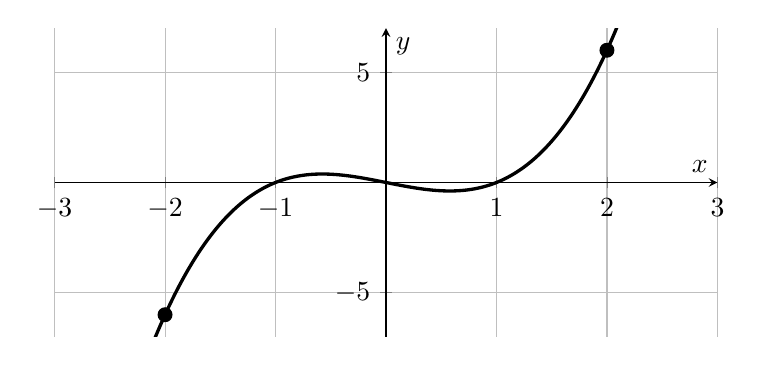
\begin{tikzpicture}
\begin{axis}[
 width=10cm,height=5.5cm,
 axis lines=middle,
 xmin=-3,xmax=3,ymin=-7,ymax=7,
 xlabel={$x$},ylabel={$y$},
 grid=both,samples=200
]
\addplot[very thick,domain=-2.2:2.2] {x^3-x};
\addplot[only marks,mark=*,mark size=2.5pt]
coordinates {(2,6) (-2,-6)};
\end{axis}
\end{tikzpicture}
\end{center}

\begin{voorbeeld}
Voor
\[
g(x)=x^3-4x
\]
geldt
\[
g(-x)=(-x)^3-4(-x)=-x^3+4x=-(x^3-4x)=-g(x).
\]
Dus \(g\) is oneven.
\end{voorbeeld}

\FVDsection{Niet elke functie is even of oneven}

De twee begrippen vormen geen volledige tweedeling.
Een functie kan ook \textbf{noch even, noch oneven} zijn.

\begin{voorbeeld}
Neem
\[
f(x)=x^2+x.
\]
Dan
\[
f(-x)=x^2-x.
\]
Dit is niet gelijk aan \(f(x)=x^2+x\), maar ook niet aan
\[
-f(x)=-x^2-x.
\]
Dus \(f\) is noch even, noch oneven.
\end{voorbeeld}

\begin{opmerking}
Om te besluiten dat een functie even of oneven is, moet de overeenkomst voor
\textbf{alle} toegelaten \(x\)-waarden gelden. Enkele symmetrisch gekozen punten
controleren kan een vermoeden opleveren, maar is geen algemeen bewijs.
\end{opmerking}

\FVDsection{Het domein hoort bij de functie}

Symmetrie vereist dat het domein zelf geschikt is.

Beschouw
\[
f(x)=x^2
\]
maar met domein
\[
[0,+\infty[.
\]

Hoewel het voorschrift \(x^2\) de bekende symmetrische parabool oproept,
is deze functie op dit domein niet even: voor bijvoorbeeld \(x=2\) behoort
\(-2\) niet tot het domein.

\begin{eigenschap}
Voor een even of oneven functie moet het domein symmetrisch zijn ten opzichte
van \(0\):
\[
x\in\operatorname{dom}f
\quad\Longrightarrow\quad
-x\in\operatorname{dom}f.
\]
\end{eigenschap}

\FVDsection{Een praktische algebraïsche test}

Om een functievoorschrift te onderzoeken:

\begin{enumerate}
  \item controleer of het domein symmetrisch is ten opzichte van \(0\);
  \item bereken \(f(-x)\);
  \item vereenvoudig;
  \item vergelijk met \(f(x)\) en \(-f(x)\).
\end{enumerate}

\[
\boxed{
\begin{array}{rcl}
f(-x)=f(x) &\Rightarrow& f\text{ is even},\\[1mm]
f(-x)=-f(x) &\Rightarrow& f\text{ is oneven},\\[1mm]
\text{anders} &\Rightarrow& f\text{ is geen van beide}.
\end{array}}
\]

\begin{voorbeeld}[Rationale functie]
Neem
\[
f(x)=\frac{x^3}{x^2-1}.
\]
Het domein is
\[
\mathbb{R}\setminus\{-1,1\},
\]
dat symmetrisch is ten opzichte van \(0\).

Verder:
\[
f(-x)=\frac{(-x)^3}{(-x)^2-1}
=\frac{-x^3}{x^2-1}
=-f(x).
\]
Dus \(f\) is oneven en haar grafiek is puntsymmetrisch ten opzichte van de oorsprong.
\end{voorbeeld}

\FVDsection{Wat kun je uit symmetrie afleiden?}

Symmetrie is geen los label. Ze laat ons nieuwe informatie afleiden.

\begin{eigenschap}[Even functie]
Als \(f\) even is en
\[
f(a)=b,
\]
dan
\[
f(-a)=b.
\]
Een nulpunt \((a,0)\) met \(a\neq0\) heeft dus ook het nulpunt
\[
(-a,0).
\]
\end{eigenschap}

\begin{eigenschap}[Oneven functie]
Als \(f\) oneven is en
\[
f(a)=b,
\]
dan
\[
f(-a)=-b.
\]
Als bovendien \(0\) tot het domein behoort, dan
\[
f(0)=0.
\]
\end{eigenschap}

Voor die laatste eigenschap:
\[
f(0)=-f(0)
\]
en dus
\[
2f(0)=0,
\qquad f(0)=0.
\]

\begin{opmerking}
De uitspraak ``elke oneven functie gaat door de oorsprong'' vereist dat \(0\)
tot het domein behoort. Bijvoorbeeld
\[
f(x)=\frac1x
\]
is oneven, maar \(0\) behoort niet tot haar domein.
\end{opmerking}

\FVDsection{Van een halve grafiek naar de volledige grafiek}

Bij een even functie volstaat de grafiek voor \(x\geq0\) om de andere helft
te reconstrueren: spiegel in de \(y\)-as.

Bij een oneven functie kunnen we eveneens uit één helft de andere afleiden:
voer een puntspiegeling in de oorsprong uit.

\begin{center}
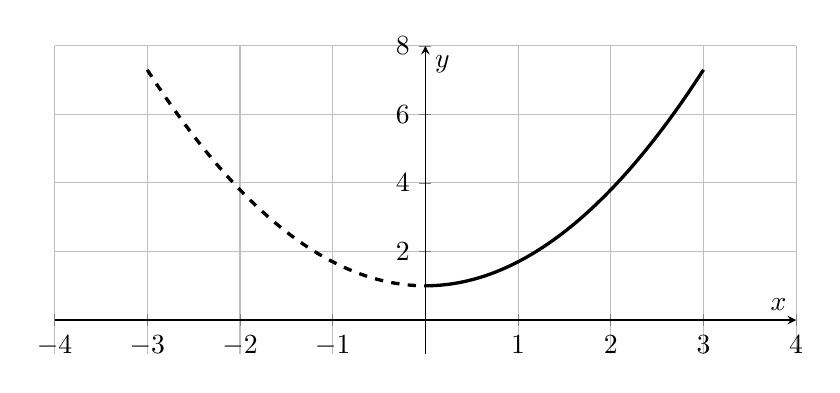
\begin{tikzpicture}
\begin{axis}[
 width=11cm,height=5.5cm,
 axis lines=middle,
 xmin=-4,xmax=4,ymin=-1,ymax=8,
 xlabel={$x$},ylabel={$y$},
 grid=both,samples=150
]
\addplot[very thick,domain=0:3] {0.7*x^2+1};
\addplot[very thick,dashed,domain=-3:0] {0.7*x^2+1};
\end{axis}
\end{tikzpicture}
\end{center}

Dit is een voorbeeld van analyseren: uit één kenmerk leiden we informatie af
over een ander deel van de grafiek.

\FVDsection{Symmetrie en andere kenmerken}

Bij een even functie komen veel kenmerken gespiegeld voor.
Als een even functie bijvoorbeeld bij \(x=a>0\) een nulpunt heeft,
dan heeft ze ook bij \(x=-a\) een nulpunt.

Bij een oneven functie worden punten
\[
(a,b)\longleftrightarrow(-a,-b)
\]
aan elkaar gekoppeld.

Ook stijgen en dalen kunnen daardoor met elkaar samenhangen.
Het is dus vaak efficiënter om eerst naar symmetrie te kijken vóór je een grafiek
volledig analyseert.

\begin{opmerking}
Symmetrie alleen bepaalt een functie niet volledig. Er bestaan oneindig veel even
en oneven functies. Ze geeft wel krachtige relaties tussen functiewaarden en
delen van de grafiek.
\end{opmerking}

\FVDsection{Onderzoeken met GeoGebra}

Voer in GeoGebra in:
\[
f(x)=x^4-3x^2,\qquad
g(x)=x^3-3x,\qquad
h(x)=x^2+x.
\]

Onderzoek voor elke functie:
\begin{enumerate}
  \item vergelijk grafisch de linker- en rechterhelft;
  \item bereken \(f(-x)\), \(g(-x)\) of \(h(-x)\);
  \item classificeer de functie als even, oneven of geen van beide;
  \item kies een punt op de rechterhelft en voorspel vanuit de symmetrie
        welk overeenkomstig punt links moet liggen;
  \item controleer je voorspelling in GeoGebra.
\end{enumerate}

\begin{opmerking}
Gebruik de grafiek om een vermoeden te vormen en het voorschrift om dat vermoeden
algemeen te verantwoorden.
\end{opmerking}

\FVDsection{Samenvatting}

\[
\boxed{
\begin{array}{ccl}
f(-x)=f(x)
&\Longleftrightarrow&
\text{even: symmetrie t.o.v. de \(y\)-as},\\[2mm]
f(-x)=-f(x)
&\Longleftrightarrow&
\text{oneven: puntsymmetrie t.o.v. de oorsprong}.
\end{array}}
\]

Onthoud:
\begin{itemize}
  \item controleer ook het domein;
  \item een functie kan even, oneven of geen van beide zijn;
  \item grafische symmetrie en algebraïsche voorwaarden beschrijven hetzelfde kenmerk;
  \item gebruik symmetrie om ontbrekende functiewaarden en grafiekdelen af te leiden;
  \item enkele gecontroleerde punten zijn geen bewijs voor een uitspraak over alle \(x\).
\end{itemize}

\end{document}
